\documentclass[11pt]{article}
\usepackage{mathblatt}
% gesetzt von werkzeuge/setzer.py (Sorte selbst) aus dem Lernweg QG4
% und den Bankzeilen; Muster bau/proben/2026-10-09/hypotenuse-muster.
\usepackage{enumitem}
\newgeometry{a4paper,margin=18mm,top=15mm,bottom=20mm,footskip=9mm}
\pagestyle{fancy}\fancyhf{}\renewcommand{\headrulewidth}{0pt}
\fancyfoot[L]{\footnotesize\color{mbgrau}QG4 \textperiodcentered{} Brüche: der Bruch als Anteil}
\fancyfoot[R]{\footnotesize\color{mbgrau}\thepage}
\setlength{\parskip}{3pt}
\renewcommand{\kreuz}[1]{\mbox{$\square$\ #1}\quad}
\newcommand{\kreuzl}[1]{\par\hangindent1.4em\hangafter1\noindent$\square$\ #1}
\newcommand{\aufg}[3]{\par\noindent\makebox[0pt][r]{#3}\begin{minipage}[t]{\linewidth}#1\end{minipage}\par}
\newcommand{\aufgg}[4]{\par\noindent\makebox[0pt][r]{#4}\begin{minipage}[t]{0.6\linewidth}\vspace{0pt}#1\end{minipage}\hfill
  \begin{minipage}[t]{0.37\linewidth}\vspace{0pt}\centering #2\end{minipage}\par}
\newcommand{\nr}[1]{\makebox[7mm][l]{\textbf{#1}}}
\newcommand{\lsg}[3]{\par\noindent\begin{minipage}[t]{9mm}\textbf{#1}\end{minipage}%
  \begin{minipage}[t]{52mm}\raggedright\bfseries\boldmath #2\end{minipage}\hspace{3mm}%
  \begin{minipage}[t]{\dimexpr\linewidth-64mm\relax}\raggedright\small #3\end{minipage}\par\vspace{4pt}}
\newlength{\kr}
\begin{document}

\noindent{\LARGE\bfseries Brüche: der Bruch als Anteil}\par\smallskip
\noindent{\small\color{mbgrau}Selbstlernheft Klasse 7 \textperiodcentered{} mit Lösungsheft \textperiodcentered{} Kennung QG4}\par\medskip
\noindent\textbf{So nutzt du das Heft:} Lies im Abschnitt das Beispiel. Rechne dann die Aufgaben der Reihe nach und vergleiche jede sofort mit dem Lösungsheft. Kreuze „kann ich“ an, wenn du die letzte Aufgabe (\emph{Ziel}) allein schaffst.\par
\noindent Mehr Aufgaben zu einem Abschnitt: Kennung deinem Nachhilfelehrer schicken (z.\,B. „QG4 mehr B“).\par\medskip
{\arrayrulecolor{mbgrau}\renewcommand{\arraystretch}{1.3}
\noindent\begin{tabular}{|>{\bfseries}p{10mm}|p{112mm}|>{\raggedleft\arraybackslash}p{10mm}|>{\centering\arraybackslash}p{14mm}|}\hline
\rowcolor{black!8} & \textbf{Abschnitt} & \textbf{Seite} & \textbf{kann ich}\\\hline
A & Anteil ablesen: Zähler und Nenner & \pageref{s:A} & $\square$\\\hline
B & Anteil einzeichnen & \pageref{s:B} & $\square$\\\hline
C & Ungleiche Teile: erst gleich groß machen & \pageref{s:C} & $\square$\\\hline
D & Bruchteil einer Zahl oder Größe berechnen & \pageref{s:D} & $\square$\\\hline
E & Anteil in Prozent & \pageref{s:E} & $\square$\\\hline
T & Probetest & \pageref{s:T} & $\square$\\\hline
\end{tabular}}\par\bigskip

\begin{tcolorbox}[colback=mbkasten,colframe=mbgrau,boxrule=0.5pt,arc=1mm,left=3mm,right=3mm,top=2mm,bottom=2mm,title={\bfseries Formel auf einen Blick},coltitle=black,colbacktitle=black!10]
\begin{minipage}[t]{0.58\linewidth}\vspace{0pt}
{\Large $\text{Anteil} = \dfrac{\text{Zähler}}{\text{Nenner}}$ \qquad $\dfrac{Z}{N}$ von $G$ \ $= G : N \cdot Z$}\par\medskip
In Worten: Der Nenner (unten) sagt, in wie viele gleich große Teile das Ganze geteilt ist. Der Zähler (oben) sagt, wie viele davon gemeint sind.\par\medskip
\textbf{So gehst du vor}\par
\nr{1}Sind alle Teile gleich groß? Sonst erst in gleich große Stücke teilen\par
\nr{2}alle Teile zählen (Nenner), gemeinte zählen (Zähler)\par
\medskip
{\small Das Ganze sind alle Teile, nicht nur die weißen. Prozent heißt Hundertstel: 50\,\% = $\frac{1}{2}$, 25\,\% = $\frac{1}{4}$, 20\,\% = $\frac{1}{5}$, 10\,\% = $\frac{1}{10}$, 75\,\% = $\frac{3}{4}$.}
\end{minipage}\hfill
\begin{minipage}[t]{0.38\linewidth}\vspace{2mm}\centering
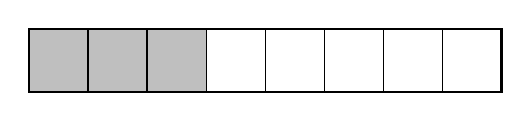
\begin{tikzpicture}[line cap=round]\fill[black!25] (0.000,0) rectangle (0.750,0.8);\draw[line width=0.4pt] (0.000,0) -- (0.000,0.8);\fill[black!25] (0.750,0) rectangle (1.500,0.8);\draw[line width=0.4pt] (0.750,0) -- (0.750,0.8);\fill[black!25] (1.500,0) rectangle (2.250,0.8);\draw[line width=0.4pt] (1.500,0) -- (1.500,0.8);\draw[line width=0.4pt] (2.250,0) -- (2.250,0.8);\draw[line width=0.4pt] (3.000,0) -- (3.000,0.8);\draw[line width=0.4pt] (3.750,0) -- (3.750,0.8);\draw[line width=0.4pt] (4.500,0) -- (4.500,0.8);\draw[line width=0.4pt] (5.250,0) -- (5.250,0.8);\draw[line width=0.9pt] (0,0) rectangle (6.0,0.8);\end{tikzpicture}
\end{minipage}
\end{tcolorbox}
\medskip\noindent\textbf{Typische Fehler – so nicht}\par\smallskip
\noindent\nr{$\times$}Teile gezählt, obwohl sie verschieden groß sind (3 von 7 Sektoren). Erst alles in gleich große Stücke teilen, dann zählen.\par
\noindent\nr{$\times$}Zähler als Anzahl gelesen: für $\frac{5}{6}$ von 24 Kästchen nur 5 gefärbt. Erst $24 : 6 = 4$, dann $4 \cdot 5 = 20$.\par
\noindent\nr{$\times$}Teil zum Rest statt zum Ganzen: 7 graue und 5 weiße Kästchen als $\frac{7}{5}$. Das Ganze sind alle 12 Kästchen: $\frac{7}{12}$.\par
\noindent\nr{$\times$}Bruch umgedreht: $2{,}8 : 3 \cdot 4$ statt $2{,}8 : 4 \cdot 3$. Immer durch den Nenner, mal Zähler.\par
\noindent\nr{$\times$}Füllmenge statt Rest angegeben. „Wie viel fehlt?“ heißt Ganzes minus Bruchteil.\par
\clearpage\label{s:A}\noindent\colorbox{black!12}{\makebox[10mm]{\Large\bfseries\strut A}}\hspace{3mm}{\Large\bfseries Anteil ablesen: Zähler und Nenner}\par\smallskip
\noindent Ein Bruch sagt, wie viel von einem Ganzen gemeint ist. Der \textbf{Nenner} (unten) zählt, in wie viele gleich große Teile das Ganze geteilt ist; der \textbf{Zähler} (oben) zählt, wie viele davon gemeint sind. Das Ganze sind \emph{alle} Teile – auch die weißen.\par\medskip
\noindent\textbf{Formel}\par\nopagebreak\noindent\hspace*{4mm}\begin{minipage}{\dimexpr\linewidth-4mm\relax}$\text{Anteil} = \dfrac{\text{gemeinte Teile}}{\text{alle Teile}}$ \qquad {\small (erst alle zählen, dann die gemeinten)}\end{minipage}\par\medskip
\noindent\textbf{Beispiel}\quad Der Streifen ist in gleich große Teile geteilt. Welcher Anteil des Streifens ist grau?\par\smallskip
\noindent\begin{minipage}[t]{0.6\linewidth}\vspace{0pt}\par\noindent\hangindent6mm\hangafter1\makebox[6mm][l]{\textbf{1}}Alle Teile zählen: 8 gleich große Teile. Das ist der Nenner.\par\smallskip\par\noindent\hangindent6mm\hangafter1\makebox[6mm][l]{\textbf{2}}Graue Teile zählen: 3. Das ist der Zähler.\par\smallskip\par\noindent\hangindent6mm\hangafter1\makebox[6mm][l]{\textbf{3}}Anteil: $\frac{3}{8}$ des Streifens ist grau.\par\smallskip\par\noindent\hangindent6mm\hangafter1\makebox[6mm][l]{\textbf{4}}Probe: 3 graue und 5 weiße Teile sind zusammen 8 – gezählt wird das Ganze, nicht nur der Rest.\par\smallskip\end{minipage}\hfill
\begin{minipage}[t]{0.37\linewidth}\vspace{0pt}\centering 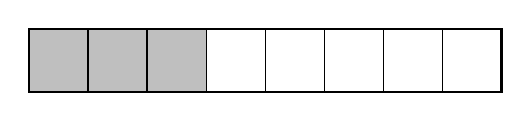
\begin{tikzpicture}[line cap=round]\fill[black!25] (0.000,0) rectangle (0.750,0.8);\draw[line width=0.4pt] (0.000,0) -- (0.000,0.8);\fill[black!25] (0.750,0) rectangle (1.500,0.8);\draw[line width=0.4pt] (0.750,0) -- (0.750,0.8);\fill[black!25] (1.500,0) rectangle (2.250,0.8);\draw[line width=0.4pt] (1.500,0) -- (1.500,0.8);\draw[line width=0.4pt] (2.250,0) -- (2.250,0.8);\draw[line width=0.4pt] (3.000,0) -- (3.000,0.8);\draw[line width=0.4pt] (3.750,0) -- (3.750,0.8);\draw[line width=0.4pt] (4.500,0) -- (4.500,0.8);\draw[line width=0.4pt] (5.250,0) -- (5.250,0.8);\draw[line width=0.9pt] (0,0) rectangle (6.0,0.8);\end{tikzpicture}\end{minipage}\par\medskip
\noindent\textbf{Aufgaben}\hspace{1em}{\small\color{mbgrau}Rechne unten im Karo. Vergleiche jede Aufgabe gleich mit dem Lösungsheft.}\par\smallskip
\aufgg{\hangindent7mm\hangafter1\nr{1.}Der Kreis ist in gleich große Teile geteilt. Welcher Anteil des Kreises ist grau?}{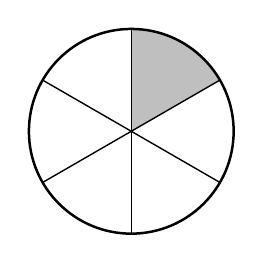
\begin{tikzpicture}[line cap=round]\fill[black!25] (0,0) -- (90:1.3) arc (90:30:1.3) -- cycle;\draw[line width=0.5pt] (0,0) -- (90:1.3);\draw[line width=0.5pt] (0,0) -- (30:1.3);\draw[line width=0.5pt] (0,0) -- (-30:1.3);\draw[line width=0.5pt] (0,0) -- (-90:1.3);\draw[line width=0.5pt] (0,0) -- (-150:1.3);\draw[line width=0.5pt] (0,0) -- (-210:1.3);\draw[line width=0.9pt] (0,0) circle (1.3);\end{tikzpicture}}{}{}
\medskip
\aufgg{\hangindent7mm\hangafter1\nr{2.}Die Figur besteht aus gleich großen Kästchen. Welcher Anteil der Figur ist grau?}{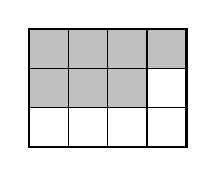
\begin{tikzpicture}[x=0.5cm,y=0.5cm,line cap=round]\fill[black!25] (0,2) rectangle (1,3);\fill[black!25] (1,2) rectangle (2,3);\fill[black!25] (2,2) rectangle (3,3);\fill[black!25] (3,2) rectangle (4,3);\fill[black!25] (0,1) rectangle (1,2);\fill[black!25] (1,1) rectangle (2,2);\fill[black!25] (2,1) rectangle (3,2);\draw[line width=0.4pt,step=1] (0,0) grid (4,3);\draw[line width=0.9pt] (0,0) rectangle (4,3);\end{tikzpicture}}{}{}
\medskip
\aufgg{\hangindent7mm\hangafter1\nr{3.}Der Streifen ist in gleich große Teile geteilt. Welcher Anteil ist grau, welcher Anteil ist weiß?}{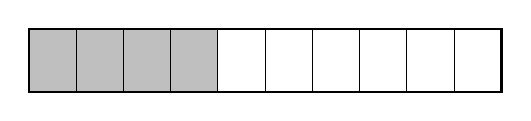
\begin{tikzpicture}[line cap=round]\fill[black!25] (0.000,0) rectangle (0.600,0.8);\draw[line width=0.4pt] (0.000,0) -- (0.000,0.8);\fill[black!25] (0.600,0) rectangle (1.200,0.8);\draw[line width=0.4pt] (0.600,0) -- (0.600,0.8);\fill[black!25] (1.200,0) rectangle (1.800,0.8);\draw[line width=0.4pt] (1.200,0) -- (1.200,0.8);\fill[black!25] (1.800,0) rectangle (2.400,0.8);\draw[line width=0.4pt] (1.800,0) -- (1.800,0.8);\draw[line width=0.4pt] (2.400,0) -- (2.400,0.8);\draw[line width=0.4pt] (3.000,0) -- (3.000,0.8);\draw[line width=0.4pt] (3.600,0) -- (3.600,0.8);\draw[line width=0.4pt] (4.200,0) -- (4.200,0.8);\draw[line width=0.4pt] (4.800,0) -- (4.800,0.8);\draw[line width=0.4pt] (5.400,0) -- (5.400,0.8);\draw[line width=0.9pt] (0,0) rectangle (6.0,0.8);\end{tikzpicture}}{}{}
\medskip
\aufg{\hangindent7mm\hangafter1\nr{4.}In einer Klasse sind 24 Kinder, 11 davon sind Jungen. Welcher Anteil der Klasse sind Mädchen?}{}{}
\medskip
\aufg{\hangindent7mm\hangafter1\nr{5.}Beim Sportfest tragen in der Klasse 7a 12 von 24 Kindern ein rotes Shirt, in der Klasse 7b 10 von 20 Kindern. In welcher Klasse ist der Anteil der roten Shirts größer? Begründe.}{}{{\scriptsize\color{mbgrau}Ziel\hspace{2mm}}}
\medskip
\par\vspace{3mm}\setlength{\kr}{\dimexpr\pagegoal-\pagetotal-10mm\relax}%
\ifdim\kr>12mm\noindent{\scriptsize\color{mbgrau}Platz zum Rechnen}\par\nointerlineskip\vspace{1mm}\noindent
\begin{tikzpicture}\clip (0,0) rectangle ({\linewidth-0.5mm},\kr);\draw[black!16,line width=0.3pt,step=5mm] (0,0) grid (\linewidth,\kr);\end{tikzpicture}\fi\par
\clearpage\label{s:B}\noindent\colorbox{black!12}{\makebox[10mm]{\Large\bfseries\strut B}}\hspace{3mm}{\Large\bfseries Anteil einzeichnen}\par\smallskip
\noindent Beim Einzeichnen zählt der Nenner, in wie viele gleiche Teile du das Ganze teilst – auch wenn die Figur mehr Kästchen hat. Rechne erst aus, wie viele Kästchen \emph{ein} Teil sind, dann nimm so viele Teile, wie der Zähler sagt.\par\medskip
\noindent\textbf{Formel}\par\nopagebreak\noindent\hspace*{4mm}\begin{minipage}{\dimexpr\linewidth-4mm\relax}Kästchen für $\frac{Z}{N}$: \ alle Kästchen $: N \cdot Z$ \qquad {\small Hat die Figur genau $N$ Teile: einfach $Z$ davon färben.}\end{minipage}\par\medskip
\noindent\textbf{Beispiel}\quad Die Figur besteht aus 12 gleich großen Kästchen. Färbe $\frac{3}{4}$ der Figur.\par\smallskip
\noindent\begin{minipage}[t]{0.6\linewidth}\vspace{0pt}\par\noindent\hangindent6mm\hangafter1\makebox[6mm][l]{\textbf{1}}Nenner 4: Das Ganze wird in 4 gleiche Teile geteilt. $12 : 4 = 3$ – ein Viertel sind 3 Kästchen.\par\smallskip\par\noindent\hangindent6mm\hangafter1\makebox[6mm][l]{\textbf{2}}Zähler 3: drei solche Teile. $3 \cdot 3 = 9$ Kästchen.\par\smallskip\par\noindent\hangindent6mm\hangafter1\makebox[6mm][l]{\textbf{3}}9 Kästchen färben (nicht 3 – der Zähler zählt Teile, nicht Kästchen).\par\smallskip\par\noindent\hangindent6mm\hangafter1\makebox[6mm][l]{\textbf{4}}Probe: 3 Kästchen bleiben weiß, das ist das letzte Viertel.\par\smallskip\end{minipage}\hfill
\begin{minipage}[t]{0.37\linewidth}\vspace{0pt}\centering 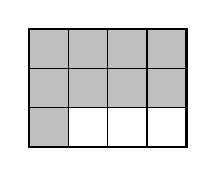
\begin{tikzpicture}[x=0.5cm,y=0.5cm,line cap=round]\fill[black!25] (0,2) rectangle (1,3);\fill[black!25] (1,2) rectangle (2,3);\fill[black!25] (2,2) rectangle (3,3);\fill[black!25] (3,2) rectangle (4,3);\fill[black!25] (0,1) rectangle (1,2);\fill[black!25] (1,1) rectangle (2,2);\fill[black!25] (2,1) rectangle (3,2);\fill[black!25] (3,1) rectangle (4,2);\fill[black!25] (0,0) rectangle (1,1);\draw[line width=0.4pt,step=1] (0,0) grid (4,3);\draw[line width=0.9pt] (0,0) rectangle (4,3);\end{tikzpicture}\end{minipage}\par\medskip
\noindent\textbf{Aufgaben}\hspace{1em}{\small\color{mbgrau}Rechne unten im Karo. Vergleiche jede Aufgabe gleich mit dem Lösungsheft.}\par\smallskip
\aufgg{\hangindent7mm\hangafter1\nr{1.}Der Streifen ist in gleich große Teile geteilt. Färbe $\frac{5}{8}$ des Streifens.}{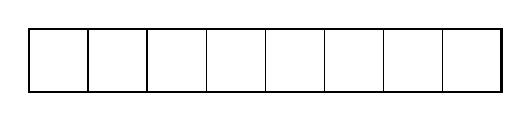
\begin{tikzpicture}[line cap=round]\draw[line width=0.4pt] (0.000,0) -- (0.000,0.8);\draw[line width=0.4pt] (0.750,0) -- (0.750,0.8);\draw[line width=0.4pt] (1.500,0) -- (1.500,0.8);\draw[line width=0.4pt] (2.250,0) -- (2.250,0.8);\draw[line width=0.4pt] (3.000,0) -- (3.000,0.8);\draw[line width=0.4pt] (3.750,0) -- (3.750,0.8);\draw[line width=0.4pt] (4.500,0) -- (4.500,0.8);\draw[line width=0.4pt] (5.250,0) -- (5.250,0.8);\draw[line width=0.9pt] (0,0) rectangle (6.0,0.8);\end{tikzpicture}}{}{}
\medskip
\aufgg{\hangindent7mm\hangafter1\nr{2.}Der Kreis ist in gleich große Teile geteilt. Färbe $\frac{2}{3}$ des Kreises.}{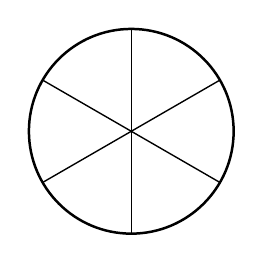
\begin{tikzpicture}[line cap=round]\draw[line width=0.5pt] (0,0) -- (90:1.3);\draw[line width=0.5pt] (0,0) -- (30:1.3);\draw[line width=0.5pt] (0,0) -- (-30:1.3);\draw[line width=0.5pt] (0,0) -- (-90:1.3);\draw[line width=0.5pt] (0,0) -- (-150:1.3);\draw[line width=0.5pt] (0,0) -- (-210:1.3);\draw[line width=0.9pt] (0,0) circle (1.3);\end{tikzpicture}}{}{}
\medskip
\aufgg{\hangindent7mm\hangafter1\nr{3.}Die Figur besteht aus 24 gleich großen Kästchen. Schraffiere $\frac{5}{6}$ der Figur.}{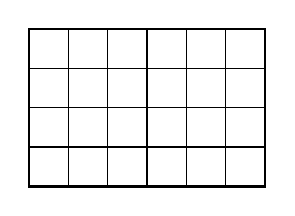
\begin{tikzpicture}[x=0.5cm,y=0.5cm,line cap=round]\draw[line width=0.4pt,step=1] (0,0) grid (6,4);\draw[line width=0.9pt] (0,0) rectangle (6,4);\end{tikzpicture}}{}{}
\medskip
\aufgg{\hangindent7mm\hangafter1\nr{4.}Die Figur zeigt ein leeres Quadrat. Kennzeichne ein Viertel seiner Fläche. Teile dazu das Quadrat zuerst in gleich große Teile.}{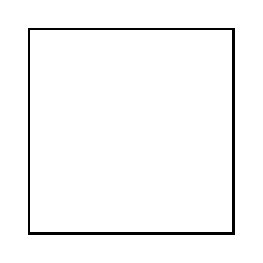
\begin{tikzpicture}\draw[line width=0.9pt] (0,0) rectangle (2.6,2.6);\end{tikzpicture}}{}{}
\medskip
\aufg{\hangindent7mm\hangafter1\nr{5.}Ein Beet hat 20 gleich große Felder. Auf $\frac{3}{5}$ der Felder sollen Tomaten wachsen, auf $\frac{1}{4}$ Salat. Reicht das Beet für beides? Wie viele Felder bleiben frei?}{}{{\scriptsize\color{mbgrau}Ziel\hspace{2mm}}}
\medskip
\par\vspace{3mm}\setlength{\kr}{\dimexpr\pagegoal-\pagetotal-10mm\relax}%
\ifdim\kr>12mm\noindent{\scriptsize\color{mbgrau}Platz zum Rechnen}\par\nointerlineskip\vspace{1mm}\noindent
\begin{tikzpicture}\clip (0,0) rectangle ({\linewidth-0.5mm},\kr);\draw[black!16,line width=0.3pt,step=5mm] (0,0) grid (\linewidth,\kr);\end{tikzpicture}\fi\par
\clearpage\label{s:C}\noindent\colorbox{black!12}{\makebox[10mm]{\Large\bfseries\strut C}}\hspace{3mm}{\Large\bfseries Ungleiche Teile: erst gleich groß machen}\par\smallskip
\noindent Zählen darfst du nur gleich große Teile. Sind die Teile verschieden groß, teile alles in Stücke von der Größe des kleinsten Teils – dann zählst du. Halbe Kästchen: in halben Kästchen zählen.\par\medskip
\noindent\textbf{Formel}\par\nopagebreak\noindent\hspace*{4mm}\begin{minipage}{\dimexpr\linewidth-4mm\relax}Nenner = Zahl der kleinsten Stücke im Ganzen \qquad Zähler = Zahl der kleinsten Stücke im grauen Teil\end{minipage}\par\medskip
\noindent\textbf{Beispiel}\quad Der Kreis ist in verschieden große Teile geteilt. Welcher Anteil des Kreises ist grau?\par\smallskip
\noindent\begin{minipage}[t]{0.6\linewidth}\vspace{0pt}\par\noindent\hangindent6mm\hangafter1\makebox[6mm][l]{\textbf{1}}Die Teile sind verschieden groß – so darf ich nicht zählen.\par\smallskip\par\noindent\hangindent6mm\hangafter1\makebox[6mm][l]{\textbf{2}}Kleinstes Stück suchen: einer der zwei kleinen Sektoren links oben. Alles in solche Stücke teilen (gestrichelt): 8 Stücke. Nenner 8.\par\smallskip\par\noindent\hangindent6mm\hangafter1\makebox[6mm][l]{\textbf{3}}Graue Stücke zählen: das große graue Stück sind 2 kleine, dazu 1 kleines: $2 + 1 = 3$. Zähler 3.\par\smallskip\par\noindent\hangindent6mm\hangafter1\makebox[6mm][l]{\textbf{4}}Anteil $\frac{3}{8}$ – nicht $\frac{2}{4}$, denn 2 von 4 Teilen wäre nur richtig, wenn alle Teile gleich groß wären.\par\smallskip\end{minipage}\hfill
\begin{minipage}[t]{0.37\linewidth}\vspace{0pt}\centering 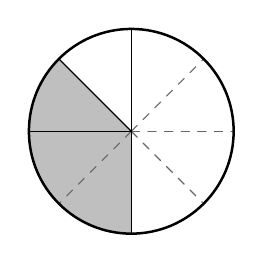
\begin{tikzpicture}[line cap=round]\fill[black!25] (0,0) -- (-90:1.3) arc (-90:-180:1.3) -- cycle;\fill[black!25] (0,0) -- (-180:1.3) arc (-180:-225:1.3) -- cycle;\draw[dashed,line width=0.4pt,black!60] (0,0) -- (0:1.3);\draw[dashed,line width=0.4pt,black!60] (0,0) -- (45:1.3);\draw[dashed,line width=0.4pt,black!60] (0,0) -- (180:1.3);\draw[dashed,line width=0.4pt,black!60] (0,0) -- (225:1.3);\draw[dashed,line width=0.4pt,black!60] (0,0) -- (270:1.3);\draw[dashed,line width=0.4pt,black!60] (0,0) -- (315:1.3);\draw[line width=0.5pt] (0,0) -- (90:1.3);\draw[line width=0.5pt] (0,0) -- (-90:1.3);\draw[line width=0.5pt] (0,0) -- (-180:1.3);\draw[line width=0.5pt] (0,0) -- (-225:1.3);\draw[line width=0.9pt] (0,0) circle (1.3);\end{tikzpicture}\end{minipage}\par\medskip
\noindent\textbf{Aufgaben}\hspace{1em}{\small\color{mbgrau}Rechne unten im Karo. Vergleiche jede Aufgabe gleich mit dem Lösungsheft.}\par\smallskip
\aufgg{\hangindent7mm\hangafter1\nr{1.}Das Rechteck besteht aus 8 Kästchen. Die schräge Linie teilt ein Kästchen in zwei Hälften. Welcher Anteil des Rechtecks ist grau?}{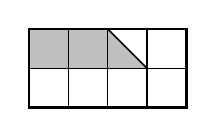
\begin{tikzpicture}[x=0.5cm,y=0.5cm,line cap=round]\fill[black!25] (0,1) rectangle (1,2);\fill[black!25] (1,1) rectangle (2,2);\fill[black!25] (2,1) -- (3,1) -- (2,2) -- cycle;\draw[line width=0.6pt] (3,1) -- (2,2);\draw[line width=0.4pt,step=1] (0,0) grid (4,2);\draw[line width=0.9pt] (0,0) rectangle (4,2);\end{tikzpicture}}{}{}
\medskip
\aufgg{\hangindent7mm\hangafter1\nr{2.}Der Kreis ist in verschieden große Teile geteilt. Welcher Anteil des Kreises ist grau?}{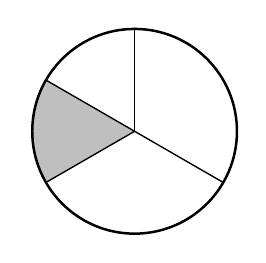
\begin{tikzpicture}[line cap=round]\fill[black!25] (0,0) -- (-150:1.3) arc (-150:-210:1.3) -- cycle;\draw[line width=0.5pt] (0,0) -- (90:1.3);\draw[line width=0.5pt] (0,0) -- (-30:1.3);\draw[line width=0.5pt] (0,0) -- (-150:1.3);\draw[line width=0.5pt] (0,0) -- (-210:1.3);\draw[line width=0.9pt] (0,0) circle (1.3);\end{tikzpicture}}{}{}
\medskip
\aufgg{\hangindent7mm\hangafter1\nr{3.}Der Kreis ist in Sektoren geteilt. Die grauen Sektoren sind markiert. Kreuze an, welcher Anteil des Kreises markiert ist.\\\par\smallskip\leftskip7mm \kreuz{$\frac{2}{5}$}\ \kreuz{$\frac{3}{8}$}\par\kreuz{$\frac{2}{8}$}\ \kreuz{$\frac{3}{5}$}}{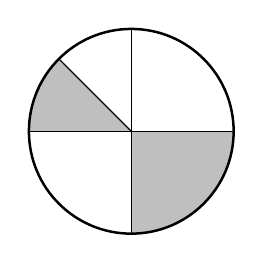
\begin{tikzpicture}[line cap=round]\fill[black!25] (0,0) -- (0:1.3) arc (0:-90:1.3) -- cycle;\fill[black!25] (0,0) -- (-180:1.3) arc (-180:-225:1.3) -- cycle;\draw[line width=0.5pt] (0,0) -- (90:1.3);\draw[line width=0.5pt] (0,0) -- (0:1.3);\draw[line width=0.5pt] (0,0) -- (-90:1.3);\draw[line width=0.5pt] (0,0) -- (-180:1.3);\draw[line width=0.5pt] (0,0) -- (-225:1.3);\draw[line width=0.9pt] (0,0) circle (1.3);\end{tikzpicture}}{}{}
\medskip
\aufgg{\hangindent7mm\hangafter1\nr{4.}Das Rechteck besteht aus 8 gleich großen Kästchen. Welcher Anteil des Rechtecks ist grau?}{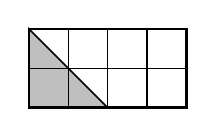
\begin{tikzpicture}[x=0.5cm,y=0.5cm,line cap=round]\fill[black!25] (0,0) -- (2,0) -- (0,2) -- cycle;\draw[line width=0.6pt] (0,0) -- (2,0) -- (0,2) -- cycle;\draw[line width=0.4pt,step=1] (0,0) grid (4,2);\draw[line width=0.9pt] (0,0) rectangle (4,2);\end{tikzpicture}}{}{}
\medskip
\aufg{\hangindent7mm\hangafter1\nr{5.}Eine Pizza wird in 6 gleich große Stücke geschnitten. Ben schneidet ein Stück noch einmal in der Mitte durch. Er isst ein ganzes Stück und ein halbes. Welchen Anteil der Pizza hat Ben gegessen? Ist das mehr als ein Viertel, weniger oder genau ein Viertel?}{}{{\scriptsize\color{mbgrau}Ziel\hspace{2mm}}}
\medskip
\par\vspace{3mm}\setlength{\kr}{\dimexpr\pagegoal-\pagetotal-10mm\relax}%
\ifdim\kr>12mm\noindent{\scriptsize\color{mbgrau}Platz zum Rechnen}\par\nointerlineskip\vspace{1mm}\noindent
\begin{tikzpicture}\clip (0,0) rectangle ({\linewidth-0.5mm},\kr);\draw[black!16,line width=0.3pt,step=5mm] (0,0) grid (\linewidth,\kr);\end{tikzpicture}\fi\par
\clearpage\label{s:D}\noindent\colorbox{black!12}{\makebox[10mm]{\Large\bfseries\strut D}}\hspace{3mm}{\Large\bfseries Bruchteil einer Zahl oder Größe berechnen}\par\smallskip
\noindent Den Bruchteil einer Zahl oder Größe rechnest du in zwei Schritten: erst durch den Nenner (das ist ein Teil), dann mal Zähler (so viele Teile). Fragt die Aufgabe, wie viel \emph{fehlt} oder \emph{übrig} ist, zieh am Ende vom Ganzen ab.\par\medskip
\noindent\textbf{Formel}\par\nopagebreak\noindent\hspace*{4mm}\begin{minipage}{\dimexpr\linewidth-4mm\relax}$\dfrac{Z}{N}$ von $G$: \ $G : N \cdot Z$ \qquad Rest $= G - \text{Bruchteil}$ \par {\small Bei Komma und Einheit: erst in die kleinere Einheit (1\,kg = 1000\,g, 1\,km = 1000\,m), wenn es dann glatter wird.}\end{minipage}\par\medskip
\noindent\textbf{Beispiel}\quad Berechne $\frac{3}{4}$ von $2{,}8$\,kg.\par\smallskip
\noindent\par\noindent\hangindent6mm\hangafter1\makebox[6mm][l]{\textbf{1}}Durch den Nenner teilen: $2{,}8 : 4 = 0{,}7$ – das ist ein Viertel.\par\smallskip\par\noindent\hangindent6mm\hangafter1\makebox[6mm][l]{\textbf{2}}Mal Zähler: $0{,}7 \cdot 3 = 2{,}1$ – drei Viertel.\par\smallskip\par\noindent\hangindent6mm\hangafter1\makebox[6mm][l]{\textbf{3}}Antwort mit Einheit: $\frac{3}{4}$ von $2{,}8$\,kg sind $2{,}1$\,kg.\par\smallskip\par\noindent\hangindent6mm\hangafter1\makebox[6mm][l]{\textbf{4}}Probe: Das Ergebnis ist kleiner als das Ganze, aber mehr als die Hälfte ($1{,}4$\,kg) – passt zu $\frac{3}{4}$.\par\smallskip\par\medskip
\noindent\textbf{Aufgaben}\hspace{1em}{\small\color{mbgrau}Rechne unten im Karo. Vergleiche jede Aufgabe gleich mit dem Lösungsheft.}\par\smallskip
\aufg{\hangindent7mm\hangafter1\nr{1.}Eine Schulstunde dauert 40 Minuten. $\frac{3}{8}$ der Stunde ist Gruppenarbeit. Wie viele Minuten sind das?}{}{}
\medskip
\aufg{\hangindent7mm\hangafter1\nr{2.}Berechne $\frac{5}{6}$ von $1{,}8$\,l. Gib das Ergebnis in Liter an.}{}{}
\medskip
\aufg{\hangindent7mm\hangafter1\nr{3.}Ein Tank fasst 80\,l. Er ist zu $\frac{3}{5}$ gefüllt. Wie viele Liter fehlen bis zur vollen Füllung?}{}{}
\medskip
\aufg{\hangindent7mm\hangafter1\nr{4.}Ein Wanderweg ist $2{,}5$\,km lang. Nach $\frac{7}{10}$ des Weges kommt eine Bank. Wie viele Meter sind das?}{}{}
\medskip
\aufg{\hangindent7mm\hangafter1\nr{5.}Eine Flasche fasst $0{,}75$\,l Saft. Lara trinkt zwei Drittel davon. Bleibt für ihren Bruder noch ein Viertelliter übrig? Begründe mit einer Rechnung.}{}{{\scriptsize\color{mbgrau}Ziel\hspace{2mm}}}
\medskip
\par\vspace{3mm}\setlength{\kr}{\dimexpr\pagegoal-\pagetotal-10mm\relax}%
\ifdim\kr>12mm\noindent{\scriptsize\color{mbgrau}Platz zum Rechnen}\par\nointerlineskip\vspace{1mm}\noindent
\begin{tikzpicture}\clip (0,0) rectangle ({\linewidth-0.5mm},\kr);\draw[black!16,line width=0.3pt,step=5mm] (0,0) grid (\linewidth,\kr);\end{tikzpicture}\fi\par
\clearpage\label{s:E}\noindent\colorbox{black!12}{\makebox[10mm]{\Large\bfseries\strut E}}\hspace{3mm}{\Large\bfseries Anteil in Prozent}\par\smallskip
\noindent Prozent heißt Hundertstel: $25\,\% = \frac{25}{100}$. Bei Figuren übersetzt du Prozent in einen Merkbruch und rechnest wie in B. Umgekehrt: Teile die Figur in Hälften, Viertel oder Fünftel und sieh nach, wie viele davon grau sind.\par\medskip
\noindent\textbf{Formel}\par\nopagebreak\noindent\hspace*{4mm}\begin{minipage}{\dimexpr\linewidth-4mm\relax}$50\,\% = \frac{1}{2}$ \quad $25\,\% = \frac{1}{4}$ \quad $20\,\% = \frac{1}{5}$ \quad $10\,\% = \frac{1}{10}$ \quad $75\,\% = \frac{3}{4}$ \qquad {\small Ein Viertel der Figur: alle Kästchen $: 4$.}\end{minipage}\par\medskip
\noindent\textbf{Beispiel}\quad Die Figur besteht aus 16 gleich großen Kästchen. Markiere $25\,\%$ der Fläche.\par\smallskip
\noindent\begin{minipage}[t]{0.6\linewidth}\vspace{0pt}\par\noindent\hangindent6mm\hangafter1\makebox[6mm][l]{\textbf{1}}Prozent in einen Bruch übersetzen: $25\,\% = \frac{25}{100} = \frac{1}{4}$.\par\smallskip\par\noindent\hangindent6mm\hangafter1\makebox[6mm][l]{\textbf{2}}Wie in B: $16 : 4 = 4$ Kästchen sind ein Viertel.\par\smallskip\par\noindent\hangindent6mm\hangafter1\makebox[6mm][l]{\textbf{3}}4 Kästchen markieren – nicht 25, so viele gibt es gar nicht.\par\smallskip\par\noindent\hangindent6mm\hangafter1\makebox[6mm][l]{\textbf{4}}Probe: 4 von 16 ist ein Viertel, und ein Viertel von 100 ist 25.\par\smallskip\end{minipage}\hfill
\begin{minipage}[t]{0.37\linewidth}\vspace{0pt}\centering 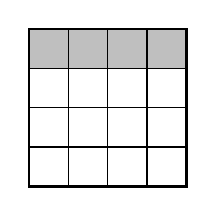
\begin{tikzpicture}[x=0.5cm,y=0.5cm,line cap=round]\fill[black!25] (0,3) rectangle (1,4);\fill[black!25] (1,3) rectangle (2,4);\fill[black!25] (2,3) rectangle (3,4);\fill[black!25] (3,3) rectangle (4,4);\draw[line width=0.4pt,step=1] (0,0) grid (4,4);\draw[line width=0.9pt] (0,0) rectangle (4,4);\end{tikzpicture}\end{minipage}\par\medskip
\noindent\textbf{Aufgaben}\hspace{1em}{\small\color{mbgrau}Rechne unten im Karo. Vergleiche jede Aufgabe gleich mit dem Lösungsheft.}\par\smallskip
\aufgg{\hangindent7mm\hangafter1\nr{1.}Der Streifen ist in gleich große Teile geteilt. Welcher Anteil des Streifens ist grau? Gib den Anteil als Bruch und in Prozent an.}{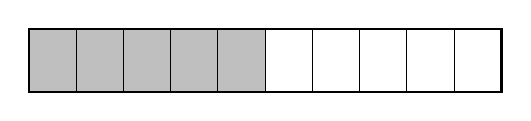
\begin{tikzpicture}[line cap=round]\fill[black!25] (0.000,0) rectangle (0.600,0.8);\draw[line width=0.4pt] (0.000,0) -- (0.000,0.8);\fill[black!25] (0.600,0) rectangle (1.200,0.8);\draw[line width=0.4pt] (0.600,0) -- (0.600,0.8);\fill[black!25] (1.200,0) rectangle (1.800,0.8);\draw[line width=0.4pt] (1.200,0) -- (1.200,0.8);\fill[black!25] (1.800,0) rectangle (2.400,0.8);\draw[line width=0.4pt] (1.800,0) -- (1.800,0.8);\fill[black!25] (2.400,0) rectangle (3.000,0.8);\draw[line width=0.4pt] (2.400,0) -- (2.400,0.8);\draw[line width=0.4pt] (3.000,0) -- (3.000,0.8);\draw[line width=0.4pt] (3.600,0) -- (3.600,0.8);\draw[line width=0.4pt] (4.200,0) -- (4.200,0.8);\draw[line width=0.4pt] (4.800,0) -- (4.800,0.8);\draw[line width=0.4pt] (5.400,0) -- (5.400,0.8);\draw[line width=0.9pt] (0,0) rectangle (6.0,0.8);\end{tikzpicture}}{}{}
\medskip
\aufgg{\hangindent7mm\hangafter1\nr{2.}Die Figur besteht aus 30 gleich großen Kästchen. Markiere $20\,\%$ der Fläche.}{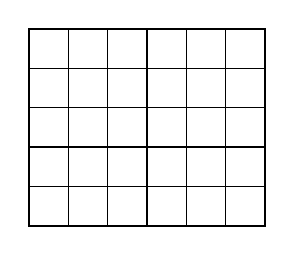
\begin{tikzpicture}[x=0.5cm,y=0.5cm,line cap=round]\draw[line width=0.4pt,step=1] (0,0) grid (6,5);\draw[line width=0.9pt] (0,0) rectangle (6,5);\end{tikzpicture}}{}{}
\medskip
\aufgg{\hangindent7mm\hangafter1\nr{3.}Die Figur besteht aus gleich großen Kästchen. Welcher Anteil der Figur ist grau? Gib den Anteil als Bruch und in Prozent an.}{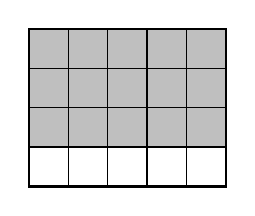
\begin{tikzpicture}[x=0.5cm,y=0.5cm,line cap=round]\fill[black!25] (0,3) rectangle (1,4);\fill[black!25] (1,3) rectangle (2,4);\fill[black!25] (2,3) rectangle (3,4);\fill[black!25] (3,3) rectangle (4,4);\fill[black!25] (4,3) rectangle (5,4);\fill[black!25] (0,2) rectangle (1,3);\fill[black!25] (1,2) rectangle (2,3);\fill[black!25] (2,2) rectangle (3,3);\fill[black!25] (3,2) rectangle (4,3);\fill[black!25] (4,2) rectangle (5,3);\fill[black!25] (0,1) rectangle (1,2);\fill[black!25] (1,1) rectangle (2,2);\fill[black!25] (2,1) rectangle (3,2);\fill[black!25] (3,1) rectangle (4,2);\fill[black!25] (4,1) rectangle (5,2);\draw[line width=0.4pt,step=1] (0,0) grid (5,4);\draw[line width=0.9pt] (0,0) rectangle (5,4);\end{tikzpicture}}{}{}
\medskip
\aufgg{\hangindent7mm\hangafter1\nr{4.}Die Figur besteht aus 20 gleich großen Kästchen. Markiere $10\,\%$ der Fläche.}{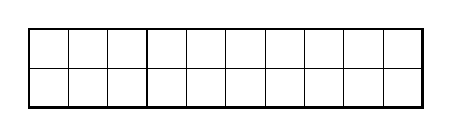
\begin{tikzpicture}[x=0.5cm,y=0.5cm,line cap=round]\draw[line width=0.4pt,step=1] (0,0) grid (10,2);\draw[line width=0.9pt] (0,0) rectangle (10,2);\end{tikzpicture}}{}{}
\medskip
\aufg{\hangindent7mm\hangafter1\nr{5.}Ein Parkhaus hat 40 Plätze, 30 davon sind besetzt. Ab $80\,\%$ Belegung zeigt die Anzeige am Eingang „fast voll“. Zeigt sie das jetzt an? Begründe mit einer Rechnung.}{}{{\scriptsize\color{mbgrau}Ziel\hspace{2mm}}}
\medskip
\par\vspace{3mm}\setlength{\kr}{\dimexpr\pagegoal-\pagetotal-10mm\relax}%
\ifdim\kr>12mm\noindent{\scriptsize\color{mbgrau}Platz zum Rechnen}\par\nointerlineskip\vspace{1mm}\noindent
\begin{tikzpicture}\clip (0,0) rectangle ({\linewidth-0.5mm},\kr);\draw[black!16,line width=0.3pt,step=5mm] (0,0) grid (\linewidth,\kr);\end{tikzpicture}\fi\par
\clearpage\label{s:T}\noindent\colorbox{black!12}{\makebox[10mm]{\Large\bfseries\strut T}}\hspace{3mm}{\Large\bfseries Probetest}\par\smallskip
\noindent Gemischt wie in der Prüfung, ohne Beispiel. Etwa 20 Minuten.\par\medskip
\noindent\textbf{Aufgaben}\hspace{1em}{\small\color{mbgrau}Rechne unten im Karo. Vergleiche jede Aufgabe gleich mit dem Lösungsheft.}\par\smallskip
\aufgg{\hangindent7mm\hangafter1\nr{1.}Die Figur besteht aus gleich großen Kästchen. Welcher Anteil der Figur ist grau? Gib den Anteil als Bruch und in Prozent an.}{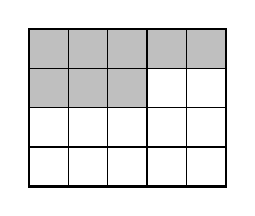
\begin{tikzpicture}[x=0.5cm,y=0.5cm,line cap=round]\fill[black!25] (0,3) rectangle (1,4);\fill[black!25] (1,3) rectangle (2,4);\fill[black!25] (2,3) rectangle (3,4);\fill[black!25] (3,3) rectangle (4,4);\fill[black!25] (4,3) rectangle (5,4);\fill[black!25] (0,2) rectangle (1,3);\fill[black!25] (1,2) rectangle (2,3);\fill[black!25] (2,2) rectangle (3,3);\draw[line width=0.4pt,step=1] (0,0) grid (5,4);\draw[line width=0.9pt] (0,0) rectangle (5,4);\end{tikzpicture}}{}{}
\medskip
\aufgg{\hangindent7mm\hangafter1\nr{2.}Der Kreis ist in Sektoren geteilt. Die grauen Sektoren sind markiert. Kreuze an, welcher Anteil des Kreises markiert ist.\\\par\smallskip\leftskip7mm \kreuz{$\frac{3}{6}$}\ \kreuz{$\frac{4}{8}$}\par\kreuz{$\frac{3}{8}$}\ \kreuz{$\frac{5}{8}$}}{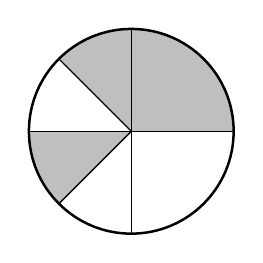
\begin{tikzpicture}[line cap=round]\fill[black!25] (0,0) -- (90:1.3) arc (90:0:1.3) -- cycle;\fill[black!25] (0,0) -- (-135:1.3) arc (-135:-180:1.3) -- cycle;\fill[black!25] (0,0) -- (-225:1.3) arc (-225:-270:1.3) -- cycle;\draw[line width=0.5pt] (0,0) -- (90:1.3);\draw[line width=0.5pt] (0,0) -- (0:1.3);\draw[line width=0.5pt] (0,0) -- (-90:1.3);\draw[line width=0.5pt] (0,0) -- (-135:1.3);\draw[line width=0.5pt] (0,0) -- (-180:1.3);\draw[line width=0.5pt] (0,0) -- (-225:1.3);\draw[line width=0.9pt] (0,0) circle (1.3);\end{tikzpicture}}{}{}
\medskip
\aufgg{\hangindent7mm\hangafter1\nr{3.}Die Figur besteht aus 25 gleich großen Kästchen. Schraffiere $\frac{3}{5}$ der Figur.}{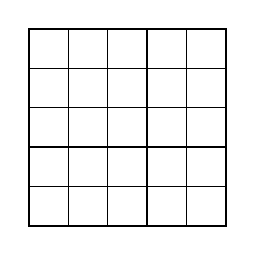
\begin{tikzpicture}[x=0.5cm,y=0.5cm,line cap=round]\draw[line width=0.4pt,step=1] (0,0) grid (5,5);\draw[line width=0.9pt] (0,0) rectangle (5,5);\end{tikzpicture}}{}{}
\medskip
\aufg{\hangindent7mm\hangafter1\nr{4.}Eine Regentonne fasst 900\,l. Sie ist zu $\frac{5}{6}$ gefüllt. Wie viele Liter passen noch hinein?}{}{}
\medskip
\aufg{\hangindent7mm\hangafter1\nr{5.}Wie viel Gramm sind $\frac{5}{8}$ von $3{,}2$\,kg?}{}{}
\medskip
\aufg{\hangindent7mm\hangafter1\nr{6.}Eine Regentonne fasst 300\,l und ist zu $\frac{4}{5}$ gefüllt. In der Nacht laufen 50\,l Regenwasser hinein. Läuft die Tonne über? Begründe mit einer Rechnung.}{}{{\scriptsize\color{mbgrau}Ziel\hspace{2mm}}}
\medskip
\par\vspace{3mm}\setlength{\kr}{\dimexpr\pagegoal-\pagetotal-10mm\relax}%
\ifdim\kr>12mm\noindent{\scriptsize\color{mbgrau}Platz zum Rechnen}\par\nointerlineskip\vspace{1mm}\noindent
\begin{tikzpicture}\clip (0,0) rectangle ({\linewidth-0.5mm},\kr);\draw[black!16,line width=0.3pt,step=5mm] (0,0) grid (\linewidth,\kr);\end{tikzpicture}\fi\par
\end{document}
